\documentclass{article}
\usepackage{amsmath}
\usepackage{graphicx}
\usepackage{hyperref}
\hypersetup{
		colorlinks=true,
		linkcolor=blue,
		filecolor=magenta,
		urlcolor=cyan,
		pdftitle={Overleaf Example},
		pdfpagemode=FullScreen,
	}
\usepackage{float}
\floatstyle{boxed} 
\restylefloat{figure}
\title{Verilog notes}
\date{01-29-2023}
\author{Tommy Bui}

\begin{document}
	\maketitle
	\newpage
	\pagenumbering{arabic}

	\tableofcontents
	\newpage

	\section{Verilog Tutorial}

	\href{https://www.chipverify.com/verilog/verilog-tutorial}{Reference to Chipverify} \newline

	\subsection{Lore}
	In the early days of integrated circuits, engineers had to physically draw transistors \& their netlist on paper. As circuits became more complex and larger in scale, this process eventually tedious. Languages such as VHDL \& Verilog were developed to simply the process of describing the functionality of IC and let tools convert the behavior into hardware using combinational \& sequential logic. \newline

	\subsection{How is Verilog useful}
	Verilog creates a level of abstraction that hides the details of its implementation \& technology. \newline

	E.g. the design of a D flip-flop requires the knowledge of the transistor layout in order to achieve an edge-triggered FF, rise/setup time, fall/clk-Q times to latch value onto flop, etc.

	\section{Introduction to Verilog}
	\href{https://www.chipverify.com/verilog/verilog-introduction}{Source}

	A digital element such as a FF can be represented using combinational gates such as NAND or NOR gates. The functionality of a FF is determined based on the layout of such gates. \underline{How the gates have to be connected is usually determined using K-maps} \newline

	Below is an schemetic of a Data flip-flop \& its corresponding truth table. The output, q is asserted only when rstn \& d are both set. \newline

	\begin{figure}[H]
		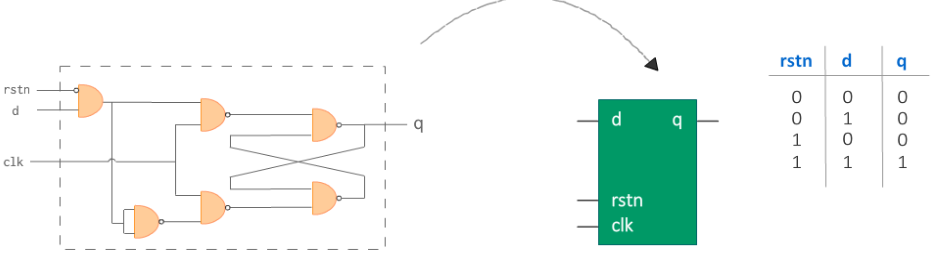
\includegraphics[width=\linewidth]{VerilogPics/figure_1.png}
		\caption{D flip flop}
		\label{D Flip-flop schematic and logic}
	\end{figure}

	\subsection{What is a hardware schematic?}

	A hardware schematic is a daigram that shows how the combinational gates should be connected to implemented a particular behaviour in hardware. From figure 1, a set of NAND gates are connected in order to create a D flip flop. 

	\subsection{What is a Hardware Description Language?}

	It's easier to describe how a block of logic should behave \& let software tools convert that behavior into an actual hardware scchematic. The langugage that describes the hardware functinality is classified as a Hardware Description Language.

	\subsection{Sections of Verilog Code}

	All behavior code should be described within the keywords module \& endmodule. 

	\subsubsection{Verilog section template}
	\begin{itemize}
		\item Module definition \& port list declaration
		\item List of input \& output ports
		\item Declaration of Verilog data types
		\item Module instantiations
		\item Behavioural code
	\end{itemize}

	\begin{figure}[H]
		
\includegraphics[width=\linewidth]{VerilogPics/figure_2.png}
		\caption{Verilog example Template}
		\label{Verilog Template}
	\end{figure}

	\section{Verilog Syntax}

	\href{https://www.chipverify.com/verilog/verilog-syntax}{Source}

\end{document}
